\documentclass{beamer}                  %printtaukseen [handout]
\usetheme{Frankfurt}
\usecolortheme{dove}

%\usepackage{pgfpages}                          %printtaukseen
%\pgfpagesuselayout{2 on 1}[a4paper,border shrink=5mm]  %printtaukseen

\usepackage[T1]{fontenc}
\usepackage[utf8]{inputenc}
\usepackage{lmodern}


%highlighting
\usepackage{color}
\newcommand{\hilight}[1]{\colorbox{yellow}{#1}}

\usepackage{mathtools}
\usepackage{xfrac}
\usepackage[finnish, british]{babel}
\usepackage{cleveref}                       %for multiple refs in one ref
%\usepackage{luximono}
\renewcommand*\familydefault{\ttdefault} %% Only if the base font of the document is to be typewriter style
\usepackage{courier}




\usepackage[style=authoryear]{biblatex} %for citations
\bibliography{/Users/omojumiller/Dropbox/Research/Dissertation/dissertation}

\DeclareMathOperator*{\E}{\mathbb{E}}               % Expectation symbol


%%%%% PATHS %%%%%

\graphicspath{{figures/}}
\usepackage{subfig} % For subfigures in floats
%\addbibresource{refs.bib} %for citations

%%%% CUSTOMIZATION OF THE TEMPLATE %%%%%

\useinnertheme{rectangles} %rectangle bullets etc
\beamertemplatenavigationsymbolsempty   %no navigation bar
\setbeamercovered{transparent}      %future bullet points transparent 
\setbeamertemplate{frametitle}[default][colsep=-4bp,rounded=false,shadow=false] %no shadows
\definecolor{dark-gray}{gray}{0.80} %color for the navigation squares

%%%% FOOTLINE CUSTOMIZATION %%%%%

\setbeamercolor{section in head/foot}{fg=black, bg=white}
\makeatletter
\setbeamertemplate{footline}
{
  \leavevmode%
  \hbox{%
  \begin{beamercolorbox}[wd=.333333\paperwidth,ht=2.25ex,dp=1ex,center]{section in head/foot}%
    \usebeamerfont{author in head/foot}\insertshortauthor~~\beamer@ifempty{\insertshortinstitute}{}{(\insertshortinstitute)}
  \end{beamercolorbox}%
  \begin{beamercolorbox}[wd=.333333\paperwidth,ht=2.25ex,dp=1ex,center]{section in head/foot}%
    \usebeamerfont{title in head/foot}\insertshorttitle
  \end{beamercolorbox}%
  \begin{beamercolorbox}[wd=.333333\paperwidth,ht=2.25ex,dp=1ex,right]{section in head/foot}%
    \usebeamerfont{date in head/foot}\insertshortdate{}\hspace*{2em}
    \insertframenumber{} / \inserttotalframenumber\hspace*{2ex} 
  \end{beamercolorbox}}%
  \vskip0pt%
}

%%%% HEADER CUSTOMIZATION %%%%%


\setbeamertemplate{mini frame}
{%
  \begin{pgfpicture}{0pt}{0pt}{.1cm}{.1cm}
    \pgfpathrectangle{\pgfpointorigin}{\pgfpoint{\the\beamer@boxsize}{\the\beamer@boxsize}}
    \pgfusepath{fill,stroke}
  \end{pgfpicture}%
}

\def\slideentry#1#2#3#4#5#6{%
  %section number, subsection number, slide number, first/last frame, page number, part number
  \ifnum#6=\c@part\ifnum#2>0\ifnum#3>0%
    \ifbeamer@compress%
      \advance\beamer@xpos by1\relax%
    \else%
      \beamer@xpos=#3\relax%
      \beamer@ypos=#2\relax%
    \fi%
  \hbox to 2pt{%
    \beamer@tempdim=-\beamer@vboxoffset%
    \advance\beamer@tempdim by-\beamer@boxsize%
    \multiply\beamer@tempdim by\beamer@ypos%
    \advance\beamer@tempdim by -.05cm%
    \raise\beamer@tempdim\hbox{%
      \beamer@tempdim=\beamer@boxsize%
      \multiply\beamer@tempdim by\beamer@xpos%
      \advance\beamer@tempdim by -\beamer@boxsize%
      \advance\beamer@tempdim by 1pt%
      \kern\beamer@tempdim
      \global\beamer@section@min@dim\beamer@tempdim
      \hbox{\beamer@link(#4){%
          \usebeamerfont{mini frame}%
          \ifnum\c@section>#1%
            \color{dark-gray}%
          \else%
            \ifnum\c@section=#1%
              \ifnum\c@subsection>#2%
                \color{dark-gray}%
              \else%
                \ifnum\c@subsection=#2%
                  \ifnum\c@subsectionslide>#3%
                    \color{dark-gray}%
                  \else%
                    \color{fg}%
                  \fi%
                \else%
                  \color{dark-gray}%
                \fi%
              \fi%
            \else%
              \color{dark-gray}%
            \fi%
          \fi%
          \usebeamertemplate{mini frame}%
        }}}\hskip-10cm plus 1fil%
  }\fi\fi%
  \else%
  \fakeslideentry{#1}{#2}{#3}{#4}{#5}{#6}%
  \fi\ignorespaces
  }
  
%%%% SOME BUG %%%%%

\def\pdftex@driver{pdftex.def}
\ifx\Gin@driver\pdftex@driver
  \def\pgfsys@color@unstacked#1{%
    \pdfliteral{\csname\string\color@#1\endcsname}%
  }
\fi

\makeatother



%%%%% INFORMATION ABOUT THE DOCUMENT %%%%%

\title[Culturally Responsive CS]{Gaining Insights Into The Effects Of Culturally Responsive Curriculum On Historically Underrepresented Students’ Desire For Computer Science}
\author[Miller]{Omoju Miller}
\institute[UC Berkeley]{University of California, Berkeley }         
                      \date{June 2016}

                      
%%%%% ACTUAL DOCUMENT PAGES %%%%%                     

\begin{document}

\section{}
        \begin{frame}[plain]
            \titlepage 
        \end{frame}

\section{Challenge}
  \begin{frame}{}
    \begin{center}
      {\LARGE Equalizing Participation in Computer Science}
      \begin{enumerate}
                \item A lack of presence of CS in K-12 education.
                \item \textcolor{red}{\textbf{The \hilight{under-production} of post-secondary degrees in CS}}. 
                \item \textcolor{red}{\textbf{The underrepresentation of \hilight{women} in CS}}.
                \item The underrepresentation of ethnic minorities in CS.
                \item A lack of positive CS role models in the media. 
                
      \end{enumerate}
    \end{center}
  \end{frame}

\section{CS10}
        \begin{frame}{}
        Three pathways into CS at UC Berkeley
            \begin{itemize}
                \item \textcolor{red}{\textbf{CS3:\hilight{Introduction to Symbolic Programming}}}.
                \item CS61A: Structure and Interpretation of Computer Programs.
                \item CS61AS: Self paced version of CS61A
            \end{itemize}
        \end{frame}

        \begin{frame}{}
        In her study of attrition in undergraduate CS at Berkeley, Lewis found that female students were disproportionately weeded out of the track, often starting at CS3 (Lewis 2010).
        \end{frame}

        \begin{frame}{}
            The Beauty and Joy of Computing
            \begin{itemize}
                 \item Uses mixture of Snap! blocks based language and python.
                 \item Re-frames CS as a tool that should be in service of society.
                 \item CS + X approach, i.e., CS + X for all X.
                 \item Prioritizes the need for students to decide their own projects.
            \end{itemize}
        \end{frame}

        \begin{frame}{}
        Three pathways into CS at UC Berkeley
            \begin{itemize}
                \item \textcolor{red}{\textbf{CS10:\hilight{The Beauty and Joy of Computing}}}.
                \item CS61A: Structure and Interpretation of Computer Programs.
                \item CS61AS: Self paced version of CS61A.

            \end{itemize}
        \end{frame}






\section{Research Methods}
\begin{frame}{}

  \begin{figure}[!htbp]
      \centering
      
      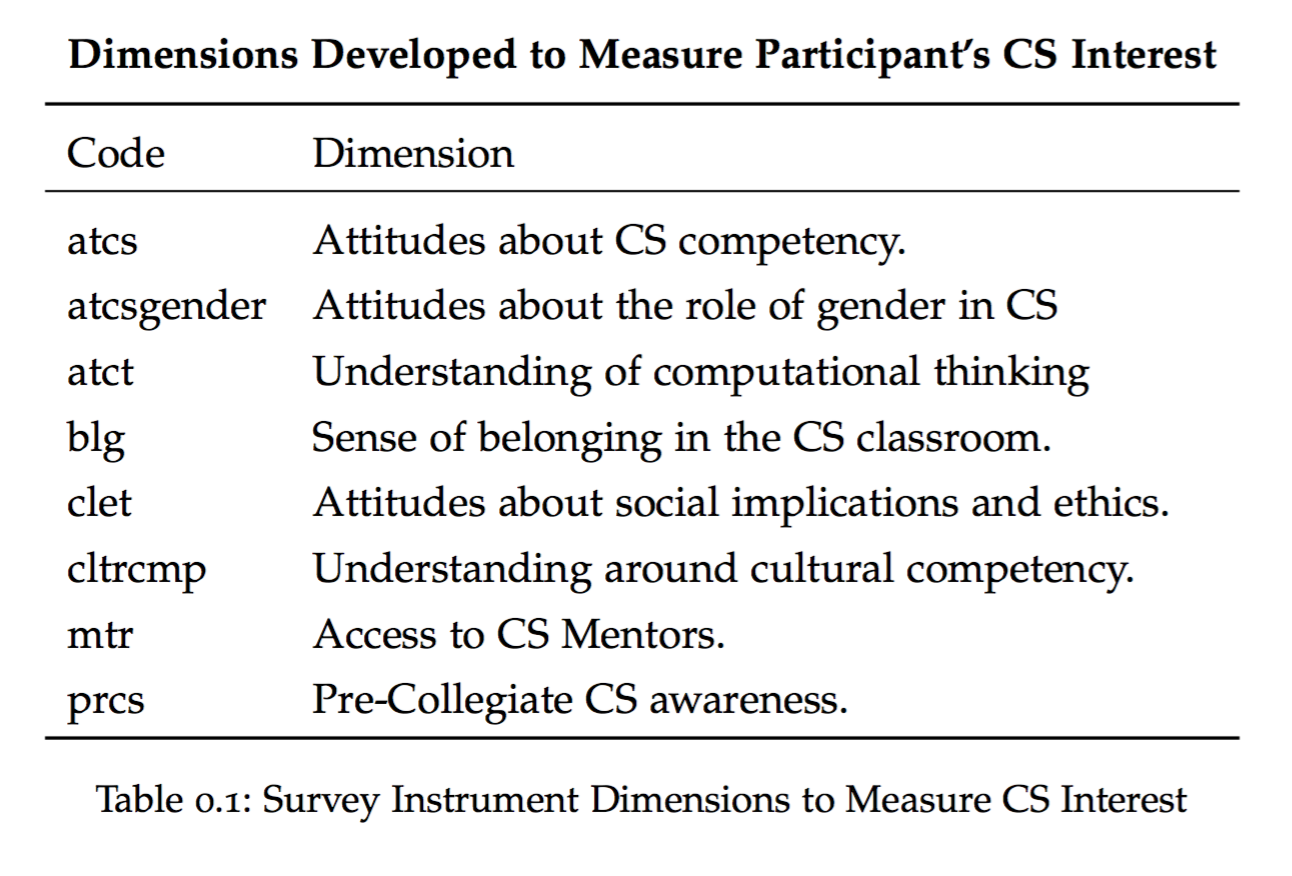
\includegraphics[width=1\textwidth]{CSAttitudes}
      
        
  \end{figure}

\end{frame}

\section{Results}
\begin{frame}{Belonging}
\begin{itemize}
\item Students generally had a stronger, statistically significant experience of belonging in CS10 as compared to CS61A. 
\item Important to notice that only around 50\% of female learners had a positive sense of belonging (\emph{p} = 0.00104) . 
\end{itemize}
\end{frame}

\begin{frame}{Effect of CS10 on CS61A Experience: Belonging}
  \begin{itemize}
  \item Students who had already taken CS10 seems to have a lower sense of belonging in CS61A, and in particular, female students, this effect seems magnified.
  \end{itemize}
\end{frame}
    
\begin{frame}{Effect of CS10 on CS61A Experience: Belonging}

  \begin{figure}[!htbp]
      \centering 
      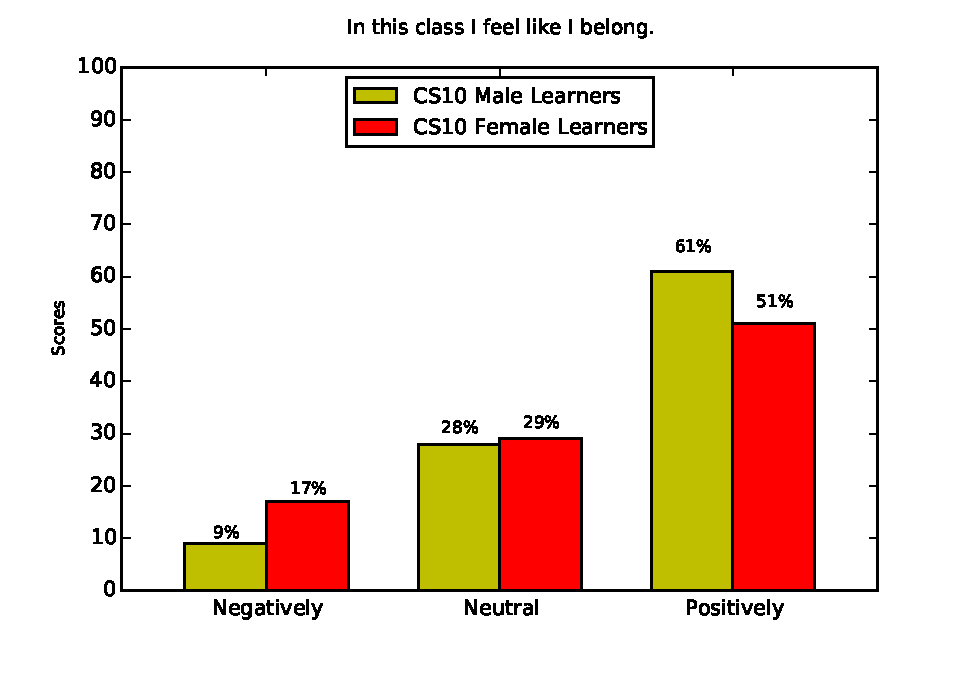
\includegraphics[width=1\textwidth]{blg_1_worstCaseScenario_cs10}
  \end{figure}

\end{frame}

\begin{frame}{Effect of CS10 on CS61A Experience: Belonging}

  \begin{figure}[!htbp]
      \centering 
      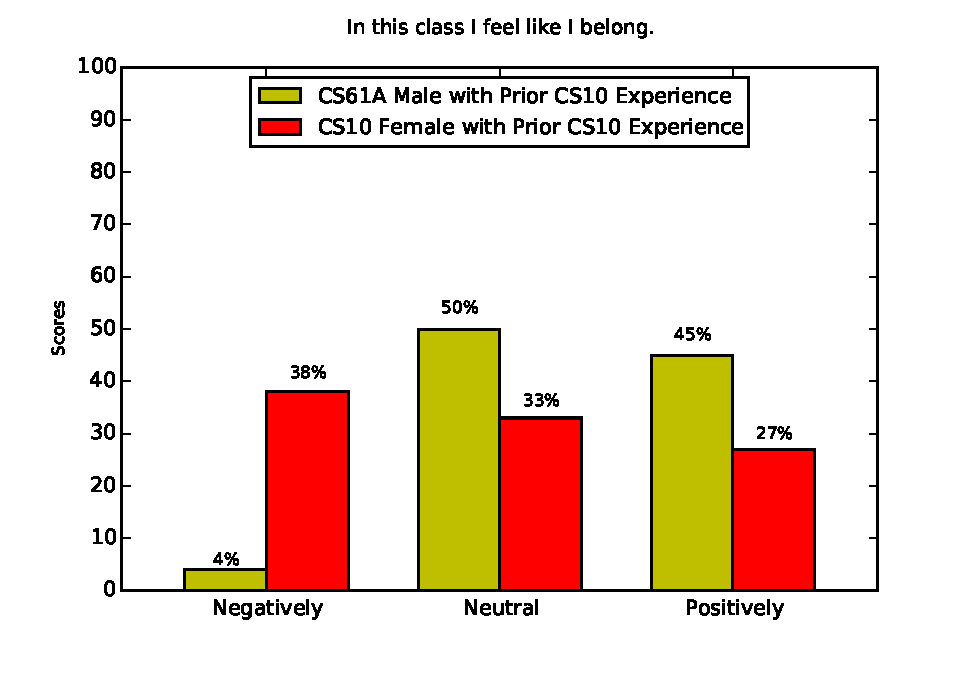
\includegraphics[width=1\textwidth]{blg_1_worstCaseScenario}
  \end{figure}

\end{frame}


\begin{frame}{What impact does CS10 have in attracting female students into the major?}

  \begin{figure}[!htbp]
      \centering
      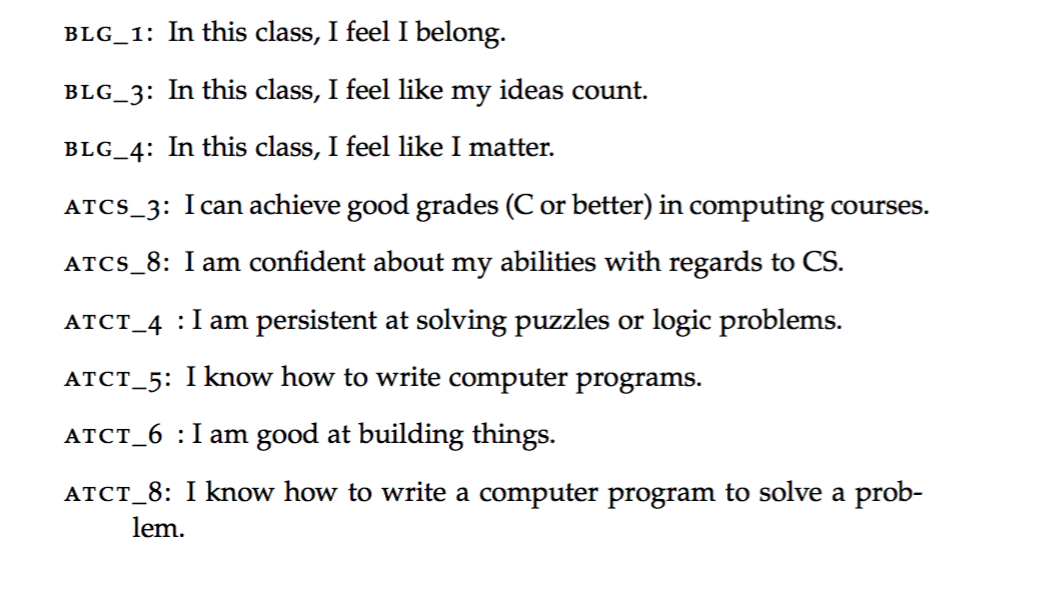
\includegraphics[width=1\textwidth]{BLG-ATCT}
      
  \end{figure}

\end{frame}

\begin{frame}{What impact does CS10 have in attracting female students into the major?}

  \begin{itemize}
  \item 
    \begin{itemize}
      \item \textbf{blg\_1}
      \item \textbf{atct\_5}
    \end{itemize}
  \item The relationship between these two variables seem to increase as girls move forward in the pipeline, as can be seen from the figures,  we are led to conclude that this relationship is truly a strong predictor of CS belonging.
  \end{itemize}

\end{frame}

\begin{frame}
  \begin{figure}[!htbp]
      \centering
      \subfloat[Female]{%
      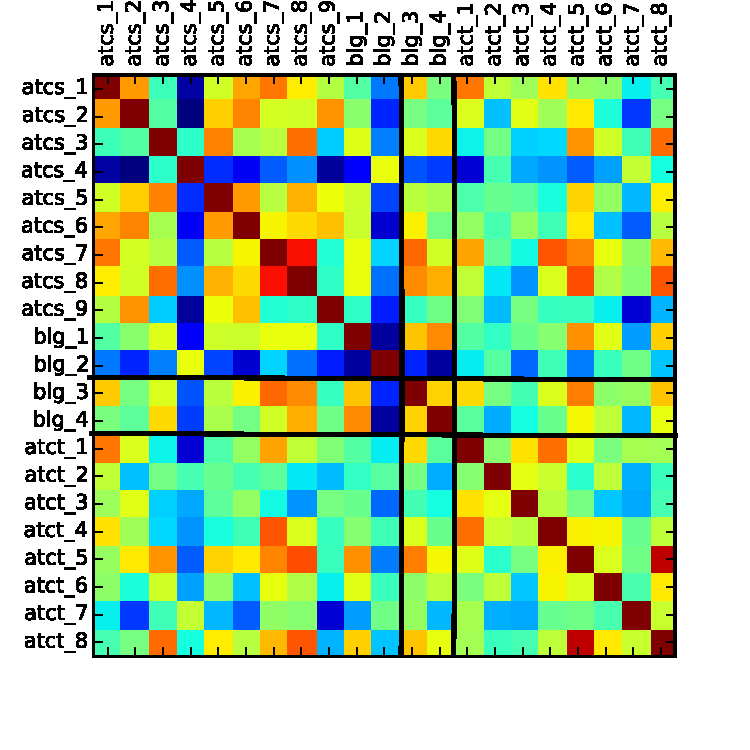
\includegraphics[width=0.5\textwidth]{priorCS10_female_corr}
      \label{corrHeatFemale}}
      \subfloat[Male]{%
      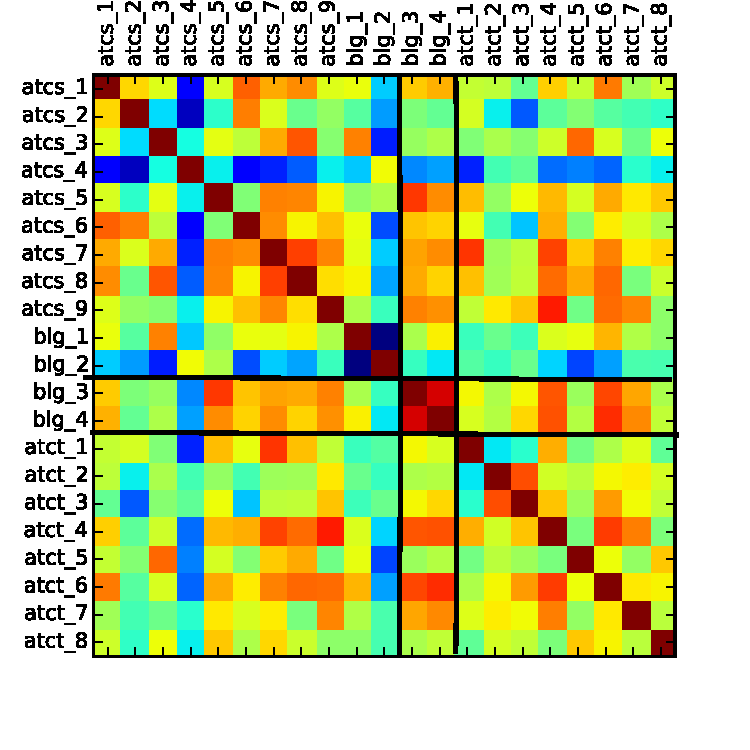
\includegraphics[width=0.5\textwidth]{priorCS10_male_corr}
      \label{corrHeatMale}}
  \caption{\textbf{Correlation matrix of CS61A students who had previously taken CS10}
  \textit{For female students \textbf{blg\_1} \& \textbf{atct\_5} are correlated. While for males we observe that it is \textbf{atct\_4} \&  \textbf{blg\_3}, and \textbf{blg\_4} \& \textbf{atct\_6}.}}
  \label{corrHeatMapFemaleCS10CS61A}
  \end{figure}
\end{frame}

\begin{frame}
  \begin{figure}[!htbp]
    \centering
    \includegraphics[width=0.6\textwidth]{cs61a_female_corr}
    \label{corr_cs61a_female}
%
\caption {\textbf{Correlation matrix for female students in CS61A at UC Berkeley}
\textit{There is a correlation between blg\_1 and atct\_5, for female students in this class. }}
\label{fig:corrFemale}
\end{figure}
\end{frame}

\section{Conclusion}

\begin{frame}{Conclusion}

  \begin{itemize}
  \item CS10 has a statistically positive effect on female students belief about CS achievement.
  \item While CS10 is successfully serving as a gateway into the major for underrepresented students, from the analysis, as great a class as CS10 is, there are still some significant environmental challenges that the overwhelmingly male environment of CS61A poses to female students sense of belonging when they advance on to 61A.
  \end{itemize}

\end{frame}


\clearpage
\end{document}
              